\chapter{Framework configurations}
\label{chap:framework_configuration}

In this chapter, we propose some configurations of the generic framework from the previous chapter. This includes configuring the meta-template for the generators, defining the prompting techniques, and defining the techniques for domain description pre-processing that the generators will use. Finally, we present a high-level architecture of the whole framework to show how these configurations can be used together.


\section{Main control instruction}

Our \emph{main control instructions} are always the same regardless of the prompting technique since the prompting techniques do not change the general task of the prompt. The table \ref{tab:main_control_instructions} shows examples of our \emph{main control instruction} configurations.


\begin{table}[!h]
    \scriptsize
    \centering
    \setlength{\tabcolsep}{0.5em}
\begin{tabular}{@{}l>{\raggedright\arraybackslash}p{0.88\textwidth}>{\raggedright\arraybackslash}p{0.5\textwidth}@{}}
    generator & main control instruction \\
    \toprule
    \addlinespace
    
$gen_c$ & Solely based on the given context extract all class names. \\
\addlinespace

$gen_a$ & Solely based on the given context generate all attributes for the class: ``\{source\_class\}''. \\
\addlinespace

$gen_{r1}$ & Solely based on the given context which associations does the class: ``\{source\_class\}'' have? \\
\addlinespace

$gen_{r2}$ & Solely based on the given context which associations are explicitly between the source class ``\{source\_class\}'' and the target class ``\{target\_class\}''? \\
\addlinespace

$gen_{cd}$ & Solely based on the given context briefly in one sentence describe only the class: ``\{source\_class\}''. \\
\addlinespace

$gen_{an}$ & Solely based on the given description and original text generate the name of the attribute of the class ``\{source\_class\}''. \\
\addlinespace

$gen_{sp}$ & Solely based on the given conceptual model summarize each given class, attribute and association. \\
\addlinespace

$gen_{sd}$ & Solely based on the given conceptual model generate descriptions only for the given classes, attributes and associations. \\
\addlinespace

	\bottomrule
	\addlinespace
	\end{tabular}
	\caption{Examples of \emph{main control instruction} configurations}
	\label{tab:main_control_instructions}
\end{table}


For the \emph{domain element generators} and the \emph{original text generator}, we refer to the inputted domain description generally as the \emph{context}. However, a more descriptive name, such as the \emph{domain description} can be used. For the name generators, we simply refer to the inputted description and original text as the \emph{description} and the \emph{original text}. Finally, for the \emph{summary generators}, we use the term \emph{conceptual model} to refer to the inputted object containing classes, attributes, and associations, but also the term \emph{domain model} can be used.

In the \emph{context specification}, we use the same input data reference name. For example, the \emph{domain element generators} and the \emph{original text generators} for the \emph{context specification} can look like this: \textit{This is the given context: ``\{domain\_description\}''} where the \textit{\{domain\_description\}} is a placeholder that is later on replaced with the user's inputted domain description.

When the task is class specific, the \emph{main control instruction} contains the \textit{\{source\_class\}} placeholder so the user's source class can be inserted. For example, this placeholder is contained by the \textit{class generator}, the \textit{association generator 1}, the \textit{class description generator}, and the \textit{attribute name generate}. Similarly, when also the target class needs to be provided, the \emph{main control instruction} contains also the \textit{\{target\_class\}} placeholder. For example, the $gen_{r2}$ contains this placeholder.

Generators such as the \emph{association generators} contain the \emph{main control instructions} in the form of a question. It should not matter if the instruction is in the form of a question or not since they both semantically are the same and the LLMs are usually trained on data both of the mentioned forms. Based on our experience, the following \emph{main control instructions} should usually lead to the same LLM output:

\begin{itemize}
\item \textit{generate all attributes for the class \{source\_class\}.}
\item \textit{which all attributes does the class \{source\_class\} have?}
\end{itemize}


\section{Output specification}


\subsection{Structured data format}

Some of the parts of the meta-template can contain data in a structured format. These data can be inserted into the prompt in many different formats such as JSON, XML, and YAML. In our configurations, we use only the JSON format, as it is one of the most popular formats for data interchange on the Internet that each LLM should be very familiar with since most of the training data for LLMs usually come from the Internet \cite{Zhao2023}.


\subsection{Automatic parsing}

For automatic output parsing, our configuration of the \emph{output specification} instructs the LLM to output the result in JSON format. To get JSON output from the LLM either a concrete JSON instance can be provided as an example or a JSON schema can be used to define the desired JSON format. For example, when the goal is to get a description of a class in JSON format from the LLM, the \emph{output specification} containing an instance of JSON format can look the following way: \\

\noindent{}\textit{Output the description in JSON format like this: \\
\{ \\
\null \quad ``description'': ``description of the class'' \\
\}} \\

\noindent{}or the \emph{output specification} instruction containing an JSON schema can look the following way: \\

\noindent{}\textit{Output the description in JSON format based on this JSON schema: \\
\{ \\
\null \quad ``\$schema'': ``http://json-schema.org/draft-04/schema\#'', \\
\null \quad  ``type'':``object'', \\
\null \quad  ``properties'': \{ \\
\null \quad \quad ``description'': \{ \\
\null \quad \quad \quad ``type'': ``string'' \\
\null \quad \quad   \} \\
\null \quad  \}, \\
\null \quad  ``required'': [ \\
\null \quad \quad   ``description'' \\
\null \quad  ] \\
\}} \\


\subsection{Faster response time}

Since it usually takes a few seconds for the LLMs to generate the complete output, instead of waiting for the whole output so the final JSON object can be parsed, the application response time can be improved by instructing the LLM to output separate JSON objects one by one so every time we need to wait only for one smaller JSON object to be generated. This can mainly help when generating domain elements as the whole output of the LLM can contain many of them. This can be done by instructing the LLM to for each outputted domain element output one JSON object, and as soon as the LLM generates some proper domain element in a JSON format, it can be parsed and displayed to the user. To achieve this, we use in the \emph{output specification} an instance of the corresponding JSON output. For example, when generating classes, the \emph{output specification} instruction can look the following way: \\

\noindent{}\textit{Output each class in JSON object like this: \{``class'': ``class name''\}.} \\

\noindent{}As a result, when the suggested classes are for example \textit{employee} and \textit{department}, instead of getting the whole output in the following single object: \\

\noindent{}\textit{\{``classes'': [\{``name'': ``employee''\}, \{``name'': ``department''\}]\}} \\

\noindent{each class is outputted in the following separate objects:} \\

\noindent{}\textit{\{``class'': ``employee''\} \\
\{``class'': ``department''\}} \\

\noindent{}Which means that these classes can be now parsed one by one.


\subsection{Output order}
\label{sec:output_order}

When humans model the domain elements solely based on a given domain description, they typically proceed in the following two steps: (1) they find the context for the given domain element, and (2) from the found context they extract the specific information such as the name of the domain element. For example, consider the following simple domain description: \\

\noindent{}\textit{In this company, every employee works in some department. Each employee is uniquely identified by his ID.} \\

\noindent{}When the task is to find associations for the class \textit{department}, usually the first step is to identify the context for this class. This context can be the first sentence of the domain description: \textit{In this company, every employee works in some department}. Subsequently, in this context the association \textit{works in} with the source class \textit{employee} and the target class \textit{department} can be found.

To mimic this approach, the \emph{output specification} can be configured the following way. For the \emph{domain element generators} for each domain element that the LLM finds, we first let the LLM to generate its original text and then its other fields such as the name. For example, the \emph{output specification} instruction for generating attributes can look like this: \\

\noindent{}\textit{Output each attribute in JSON object like this: \\
\{``originalText'': ``copy the part of the given context containing \\ this attribute'', ``name'': ``attribute name''\}.} \\

\noindent{}As we can see, for each attribute first the original text and then the name is generated. Also, notice that the LLM is instructed to output a single JSON object for each attribute as discussed earlier.



\section{Prompting techniques}

In this section, we describe our configurations of the \emph{modeling procedure}, \emph{example specification}, \emph{context specification}, and additional configurations of the \emph{output specification} as all these parts depend on the used prompting technique.

For each generator, we have a baseline configuration where no prompting technique is used. Additionally, for generators of classes, attributes, and associations, we introduce configurations that use the following prompting techniques:

\begin{itemize}
\item CoT
\item N-shot
\item CoT + N-shot
\end{itemize}

\noindent{}And, for the \emph{class generator}, we implemented the ToT approach. Now follows a more detailed description of these configurations.


\subsection{Chain of thoughts}

First, we need to come up with reasoning steps that the LLM can generate before outputting each domain element. Some possible reasoning steps can be generated by the LLM by adding the \textit{Let's think step by step} phrase into the \emph{modeling procedure} as discussed in the section \ref{sec:chain_of_thoughts}. Figure \ref{fig:cot-think-step-by-step} shows one of the possible reasoning steps when using ChatGPT-4o to generate attributes with a simple domain description.

\begin{figure}[!h]
    \centering
    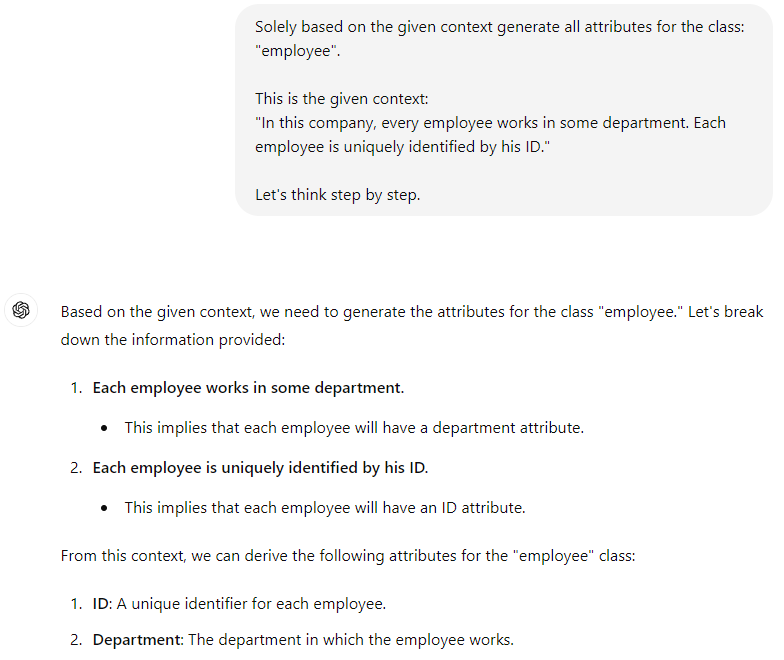
\includegraphics[scale=0.6]{img/cot-think-step-by-step.png}
    \caption{\centering Example of automatically generated reasoning steps by ChatGPT-4o for finding attributes in a simple domain description}
    \label{fig:cot-think-step-by-step}
\end{figure}

As we can see, ChatGPT-4o for each attribute first rephrased some parts of the domain description, and then, based on these parts identified the possible attributes. Note that this approach is consistent with the output order that we specified in the section \ref{sec:output_order}.

Inspired by this result, we implemented a simple CoT strategy that instructs the LLM to first generate for each domain element its original text, then generate all other fields such as the name and at the end generate all these previous items in a single JSON object. Our goal is to force the LLM to generate the original text and then mainly based on this original text generate the other fields of the corresponding domain element.
The table \ref{tab:cot-prompt-templates} shows our \emph{modeling procedures} and the \emph{output specifications} for each \emph{domain element generators}.

The LLM is instructed to first output for each domain element its context which, is the original text then output its name, and for the associations to also output its source class and its target class. After that, the LLM is instructed to generate the final JSON object with all these mentioned fields so that the output can be automatically parsed.

% Other more sophisticated CoT strategies can be used. For example, when the LLM generates attributes to instruct the LLM to add for each generated domain element a reason why it thinks it is an attribute.

\begin{table}[!h]
    \scriptsize
    \centering
    \setlength{\tabcolsep}{0.5em}
\begin{tabular}{@{}l>{\raggedright\arraybackslash}p{0.35\textwidth}>{\raggedright\arraybackslash}p{0.52\textwidth}@{}}
        generator & modeling procedure & output specification \\
    \toprule
    \addlinespace
$gen_c$ & For each class copy the part of the given context containing this class and output its name and then output this class in JSON object. & The output should look like this: \newline
context: copy the part of the given context containing this class \newline
name: class name \newline
JSON object: \{``originalText'': ``copy the part of the given context containing this attribute'', ``name'': ``class name''\}. \\
\addlinespace

$gen_a$ & For each attribute copy the part of the given context containing this attribute and output its name and then output this attribute in JSON object. & The output should look like this: \newline
context: copy the part of the given context containing this attribute \newline
name: attribute name \newline
JSON object: \{``originalText'': ``copy the part of the given context containing this attribute'', ``name'': ``attribute name''\}. \\
\addlinespace

$gen_{r1}$ & For each association copy the part of the given context containing this association and output its name, source class, target class and then output this association in JSON object. &
The output should look like this: \newline
context: copy the part of the given context containing this association \newline
name: association name \newline
source class: source class name \newline
target class: target class name \newline
JSON object: \{``originalText'': ``copy the part of the given context containing this association'', ``name'': ``association name'', ``source'': ``source class name'', ``target'': ``target class name''\} \\
\addlinespace

$gen_{r2}$ & For each association copy the part of the given context containing this association and output its name, source class, target class and then output this association in JSON object. &
The output should look like this: \newline
context: copy the part of the given context containing this association \newline
name: association name \newline
source class: \{source\_class\} \newline
target class: \{target\_class\} \newline
JSON object: \{``originalText'': ``copy the part of the given context containing this association'', ``name'': ``association name'', ``source'': ``\{source\_class\}'', ``target'': ``\{target\_class\}''\} \\

	\addlinespace
	\bottomrule
	\addlinespace
	\end{tabular}
	\caption{Example of CoT \emph{modeling procedure} and \emph{output specification} configurations}
	\label{tab:cot-prompt-templates}
\end{table}


\subsection{N-shot prompting}

We use examples based on the domain description and its domain model that is shown in the figure \ref{fig:prompting-domain}.

\begin{figure}[!h]
    \centering
    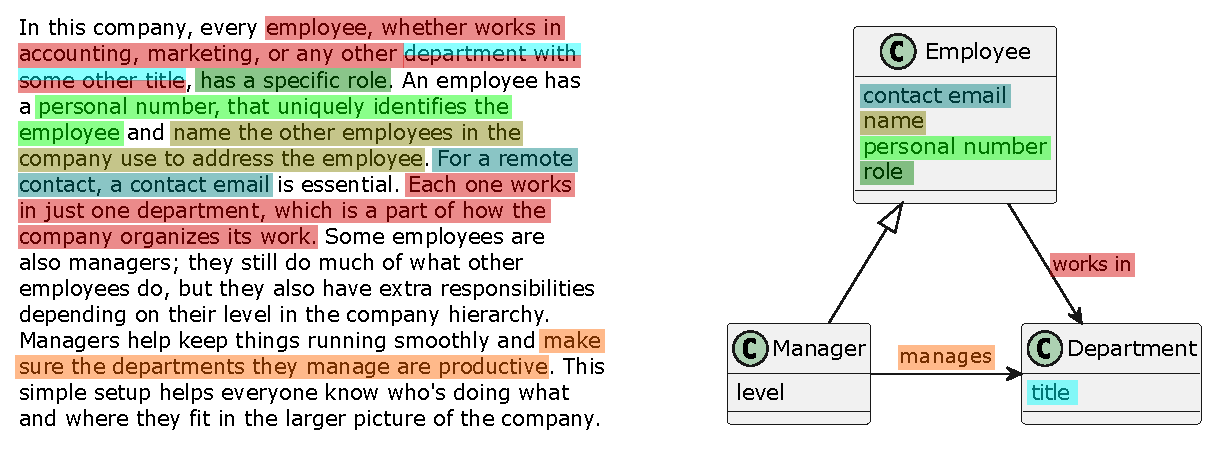
\includegraphics[scale=0.6]{img/prompting-domain.pdf}
    \caption{\centering The simple company employees domain description and its corresponding domain model used for N-shot prompting in \emph{domain element generators}}
    \label{fig:prompting-domain}
\end{figure}

For the \emph{class generator}, we use the three classes as examples. The \emph{example main control instruction} is \textit{Solely based on the given context extract all class names}, the \emph{example context specification} contains the complete domain description from the figure \ref{fig:prompting-domain} and the \emph{context specification} is the following: \\

\noindent{}\textit{\frenchspacing\{``name'': ``employee''\} \\
\{``name'': ``department''\} \\
\{``name'': ``manager''\}} \\

For the \emph{attribute generator}, we use the colored attributes, each with the colored part of the text as examples of the corresponding original texts. For example, for the class \textit{employee} the \emph{example main control instruction} is \textit{generate all attributes for the class: ``employee''}, the \emph{example context specification} contains only the parts of domain description that provide information about the class \textit{employee} and its attributes like this: \\

\noindent{}\textit{In this company, every employee, whether works in accounting, marketing, or any other department with some other title, has a specific role. An employee has a personal number, that uniquely identifies the employee and name the other employees in the company use to address the employee. For a remote contact, a contact email is essential.} \\

\noindent{}And the \emph{context specification} is the following: \\

\noindent{}\textit{\frenchspacing\{``originalText": ``has a specific role'', ``name'': ``role''\} \\
\{``originalText'': ``personal number, that uniquely identifies the employee'', ``name'': ``personal number''\} \\
\{``originalText'': ``name the other employees in the company use to \\ address the employee'', ``name'': ``name''\} \\
\{``originalText'': ``For a remote contact, a contact email'', ``name'': ``contact email''\}} \\


For \emph{association generators}, we proceed similarly, but for \emph{association generator 1} we provide each sample association twice, first for the source class and then for the target class. For example, the association \textit{works in} with the source class \textit{employee} and the target class \textit{department} is used as one example with the following \emph{example main control instruction}: \\

\noindent{}\textit{Solely based on the given context which associations does the class: ``\textbf{employee}'' have?} \\

\noindent{}and the second time with the following \emph{example main control instruction}: \\

\noindent{}\textit{Solely based on the given context which associations does the class: ``\textbf{department}'' have?} \\

\noindent{}In both cases, the \emph{example context specification} and the \emph{context specification} is the same.

Furthermore, concrete examples can be used to specify the output text format. For example, when the LLM is not provided with a specific name format for the corresponding domain elements, the outputted names can sometimes be in a snake case convention and some other time in a camel case convention. But when the provided examples contain a consistent naming format, the LLM usually outputs the provided format consistently. Similarly, the N-shot prompting technique lets us specify the naming style. For example, when no naming style is provided for attributes, they can contain some unwanted words such as starting with the word \textit{has} which is more common for association names.


\subsection{CoT + N-shot prompting}

Our combination of the CoT and the N-shot prompting technique contains the same \emph{modeling procedure} as shown in the table \ref{tab:cot-prompt-templates} for the CoT only approach. However, the \emph{output specification} contains only the instance of the expected JSON object and the intermediate steps are demonstrated in the \emph{example context specification} where the $N$ examples are provided. For example, the labeled example for the attribute \textit{role} of the class \textit{employee} looks like this: \\

\noindent{}\textit{context: has a specific role} \\
\textit{name: role} \\
\textit{JSON object: \{``originalText'': ``has a specific role'', ``name'': ``role''\}} \\

\noindent{}And the labeled example for the association \textit{manages} with the source class \textit{manager} and the target class \textit{department} looks like this: \\

\noindent{}\textit{context: make sure the departments they manage are productive} \\
\textit{name: manages} \\
\textit{source class: manager} \\
\textit{target class: department} \\
\textit{JSON object: \{``originalText'': ``make sure the departments they manage are productive'', ``name'': ``manages'', ``source'': ``manager'', ``target'': ``department''\}}


\subsection{Tree of thoughts}

Even though our defined generators do not solve any typical complex tasks that the ToT is usually used for, we try to use this prompting technique for the \emph{class generator} in the single prompt format as discussed in the section \ref{sec:tree_of_thoughts}. We use the mentioned single-prompt phrase in the \emph{modeling procedure} but we slightly edited it to fit our meta-template structure: \\

\noindent{}\textit{Imagine three different experts are \textbf{solving the given task}. All experts will write down 1 step of their thinking, then share it with the group. Then all experts will go on to the next step, etc. If any expert realises they are wrong at any point they leave.} \\

\noindent{}The bold text highlights the changes we made to the original phrase of the ToT prompting technique. Also, we removed the last sentence from the original phrase which is the following: \textit{The question is}. Figure \ref{fig:meta-templates} shows an abbreviated example of a generated output with the \emph{Llama-3-70B} LLM for \textit{aircraft manufacturing}\footnote{\url{https://github.com/dataspecer/domain-modeling-benchmark/blob/d9e00b65a376dbefe5b605bd680621f9f63f9252/manual\%20evaluation\%20domains/aircraft\%20manufacturing/domain-description-02.txt}} domain description.


\begin{figure}[!h]
    \centering
\begin{lstlisting}[
  basicstyle=\ttfamily\scriptsize,
  breaklines=true,
  keywordstyle=\ttfamily,
  stringstyle=\ttfamily,
  showstringspaces=false,
  upquote=true,
  stringstyle=
]
01 Expert 1:
02 My first step is to identify the main entities mentioned in the context. Based on the text, I think the following classes can be extracted:
03 {"name": "Party"}
04 {"name": "Customer"}
05 {"name": "Supplier"}
...
11 Expert 2:
12 I agree with Expert 1, but I also think we can extract another class:
13 {"name": "Purchase"}
14 Expert 3:
15 I'm not sure about "Purchase" yet, but I think we can also extract:
16 {"name": "DesignModel"}
...
31 Expert 3:
32 I'm starting to think that "DesignModel" might not be a separate class, but rather an attribute of "PartModel". However, I do agree with the other experts' analysis.
...
47 Expert 3:
48 I'm out. I was wrong about "DesignModel" being a separate class.
...

\end{lstlisting}
    \caption{\centering Prompt meta-template for the generators}
    \label{fig:meta-templates}
\end{figure}



As we can see, first, the LLM created a preliminary list of classes (lines 01 -- 05) then, it added classes that seemed to be missing (lines 11 -- 13) and then it reasoned about the classes it was not certain about (lines 31 and 32). In this step, the class \textit{DesignModel} was removed as the LLM thought that it is rather an attribute of the class \textit{PartModel} which is valid reasoning. In the end, one of the experts left since at the start he suggested an incorrect class (lines 47 and 48). \\

We do not experiment with any iterative prompting technique as this would significantly increase the response time of our application as discussed in the section \ref{sec:iterative_prompting}.

All our prompt templates with the mentioned configurations can be found in our GitHub repository\footnote{\url{https://github.com/Dominik7131/Conceptual-Modeling-LLM-Assistant/tree/master/prompts}}.


\section{Domain description pre-processing}

\subsection{Motivation}

From our observation, when an LLM works with longer domain descriptions it can mainly make the following two mistakes:

\begin{enumerate}
\item extract irrelevant domain elements from irrelevant parts of the domain description
\item skip some important parts of the domain description that contain some important domain elements
\end{enumerate}


To mitigate these issues, the domain description can be simplified and the unimportant parts of the domain description can be removed based on the given task with techniques such as retrieval-augmented generation. Ideally, this would solve both of these issues since the LLM could not work with irrelevant parts of the domain description as they would not be present in the prompt thus the LLM would focus only on the important parts of the domain description.
Furthermore, these approaches can reduce the prompt length which can help when working with a domain description that does not fit in the context window of the LLM.

%Our goal is to improve the LLM performance by pre-processing the domain description. The pre-processing can be done either only once after the user inputs his domain description or it can be done before using each generator for providing only the relevant information that are needed for solving the given task.


\subsection{Domain description simplification}

After the user inputs his domain description, it can be simplified by the LLM, and subsequently, all the \emph{text to model generators} can work only with this simplified version. However, there are a few disadvantages to this approach.

First, the LLM sometimes changes some names of the original domain elements. For example, when we instructed the ChatGPT-4o with a domain description about \emph{aircraft manufacturing} and with the following prompt: \\

\noindent{}\textit{Simplify each sentence structure in the following text. Make sure to not change any nouns and verbs as we want to keep the names of all domain elements unchanged. This is the following text: ``The domain centers around the manufacturing and distribution of aircraft \ldots''.} \\

\noindent{}The sentence \textit{Customers represent the clients who purchase the finished aircraft.} was simplified into \textit{Customers are clients who buy finished aircraft.} This means that the original association name \textit{client purchases aircraft} was changed into \textit{client buys aircraft} which is semantically the same but it can be a problem if the user wants the suggestions to have the same name as described by his domain description.

The second disadvantage is that the domain description simplification removes the ability to highlight the original text for each suggested domain element in the original description since the LLM works only with the simplified version of the domain description. Therefore, we do not simplify the domain description.


\subsection{Retrieval-augmented generation}


When the domain description is segmented into chunks and when each chunk is considered as one of the documents of the external knowledge, the RAG technique can be used for filtering domain description, i.e. removing unnecessary parts of the domain description based on the given task. For example, consider the following domain description: \\

\noindent{}\textit{In this company, every employee works in some department. Each employee is uniquely identified by his ID.}\\

\noindent{}When the goal is to extract attributes or associations of the class \textit{department}, we are only interested in the first sentence since this is the only sentence that contains information about this class. Therefore, in this case, we can provide only the first sentence of the domain description into the \emph{context specification} of the prompt template. In other words, the first sentence can be the first chunk, and the second sentence can be the second chunk subsequently, the second chunk can be removed as it does not contain information about the given class.


\subsubsection{Work-flow}
\label{sec:RAG_work_flow_dd}

In the indexing phase, the domain description is segmented into chunks that can be embedded into vectors by an embedding model and cached into a database. In the retrieval phase, some technique is applied for chunks classification to determine which chunks are relevant based on the given task. And finally, in the generation phase, the relevant chunks are assembled together to create a new domain description.


\subsubsection{Configurations}
\label{sec:rag_configurations}

We use the mentioned RAG technique for the generators of attributes, associations, descriptions, data types, and cardinalities since in these cases only the information about the source class $C$ is needed to generate the correct output.

At first, we considered using LLM to directly output the relevant texts from the domain description based on the given source class. However, this process can take a long time as in the worst-case scenario the LLM has to copy the whole domain description to the output. Instead, we implemented a semantic and a syntactic approach.

%The semantic approach uses an embedding model that converts each domain description chunk into a vector space to create the external knowledge base. Subsequently, the sentence ``\emph{Info about \{source\_class\}}'' where the \textit{\{source\_class\}} placeholder is replaced by the given class name is embedded by the same model and similar chunks from the external knowledge base are retrieved and then used to build a new domain description.

The semantic approach uses an embedding model that converts each domain description chunk into a vector space to create the external knowledge base. Subsequently, the given source class name is embedded by the same model, and similar chunks from the external knowledge base are retrieved and then used to build a new domain description.

The syntactic approach uses a language model that converts each domain description chunk into lemmas. Subsequently, the given source class is converted into lemmas by the same model, and the chunks that contain the exact lemmas as the given source class are retrieved from the external knowledge base and then used to build a new domain description.


\subsubsection{Example}

Consider the source class \textit{department} and the following domain description where the first sentence is the first chunk and the second sentence is the second chunk: \\

\noindent{}\textit{In this company, every employee works in some department. Each employee is uniquely identified by his ID.} \\

For the semantic approach, each sentence is embedded into a vector and its similarity is compared with the source class \textit{department} that is also converted into a vector by the same embedding model. Then, the first sentence is most probably classified as relevant since it contains the class \textit{department}, and the second sentence is probably classified as irrelevant since it does not contain any information similar to the \textit{department}.

For the syntactic approach, first, each word in the domain description is converted into the following lemmas: \\

\noindent{}\textit{In this company, every employee \textbf{work} in some department. Each employee \textbf{be} uniquely \textbf{identify} by his ID.} \\

\noindent{}The bold words emphasize the differences between the original domain description and the domain description where each word is converted into a lemma. Then, each word in the given source class \textit{department} is converted into a lemma which in this case is the same word \textit{department}.  In this case, only the first chunk is relevant since it contains the word \textit{department}. We do not enforce the chunk to contain the lemmas in the same order as the given source class. For example, consider the source class \textit{registration application} and the following chunk: \\

\noindent{}\textit{Application of registration needs to be provided.} \\

\noindent{}If the strict lemmas order was enforced then this chunk would be classified as irrelevant for the source class \textit{registration application} which is an undesired behavior.


\section{High-level architecture}
\label{sec:high_level_architecture}

Now we describe the reference high-level architecture of the framework. The framework should consist of the frontend and the backend. The frontend should communicate with the backend that should implement the LLM assistant services and should provide them via API. To support our proposed configurations, the backend should contain at least the following components:

\begin{itemize}
\item \emph{RAG processor} for filtering a domain description based on the given class name
\item \emph{prompt manager} for fetching the corresponding prompt template with the corresponding prompt technique based on the user input
\item \emph{placeholder replacer} for replacing all placeholders in the prompt template with the input from the user
\item \emph{LLM manager} for sending the prompt to the LLM and parsing the output
\end{itemize}


\subsection{Work-flow}

Figure \ref{fig:work-flow} shows an overview of the architecture work-flow which can be described in the following way. On the frontend through the user interface, the users should be able to insert their input and then call some service provided by the backend. When the backend is called typically some generator is executed. First, for the \emph{text to model generators} the domain description can be filtered using some RAG technique implemented by the \emph{RAG processor} component. Then, the corresponding prompt template with the selected prompt engineering technique should be retrieved by the \emph{prompt manager}. Subsequently, in the prompt template, all the prompt placeholders should be replaced by the \emph{placeholder replacer} component. Then, the assembled prompt should be sent by the \emph{LLM manager} to some LLM and the output should be parsed, and then the parsed output can be checked for mistakes. The approved parsed output should be then sent to the frontend and displayed to the user.

\begin{figure}[!h]
    \centering
    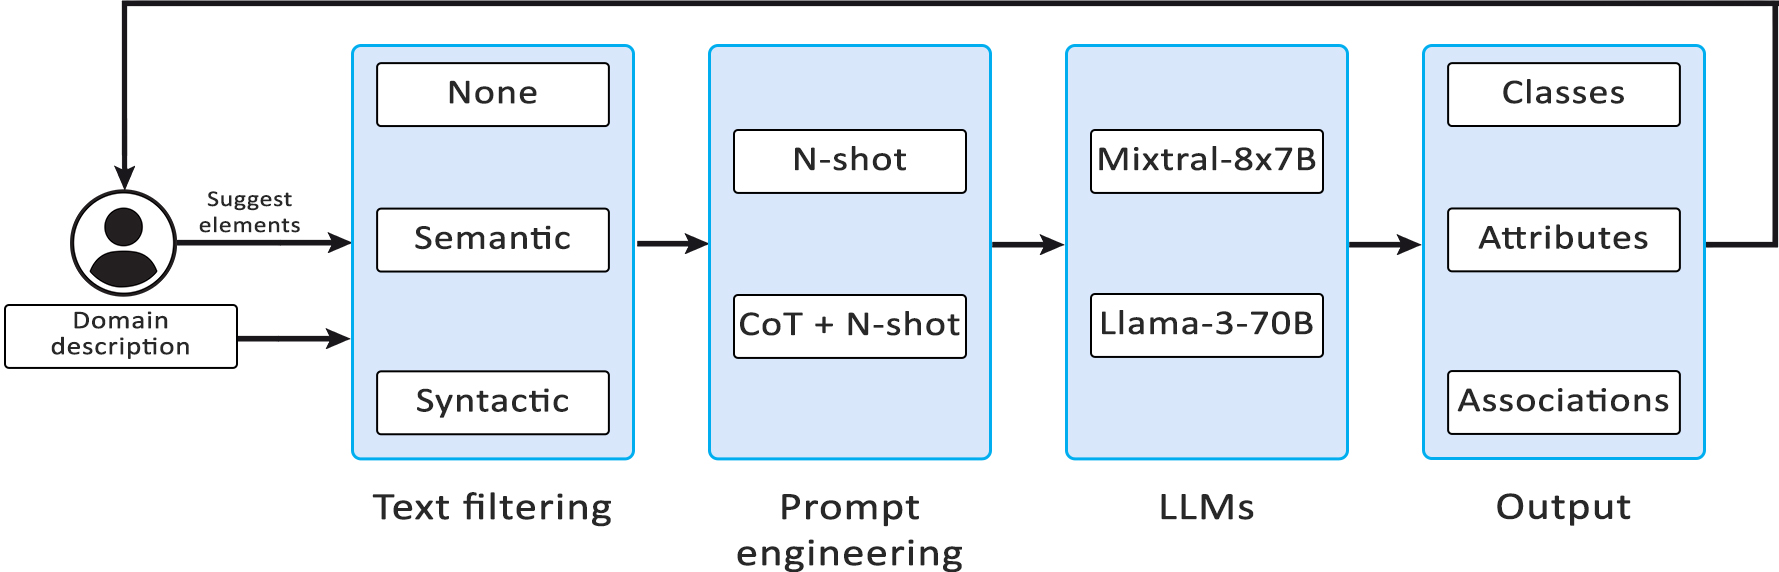
\includegraphics[scale=0.23]{img/work-flow.jpg}
    \caption{\centering Schema of the flow of processing the textual domain description}
    \label{fig:work-flow}
\end{figure}
